%!TEX root = main.tex

\section{Introduction}

The previous chapter introduced a pair of new algorithms that incorporated compliance information and proved that they preserved the worst case performance guarantees up to multiplicative factors.
This leaves open the question as to whether these new algorithms can in fact outperform their standard counterparts in practical settings. 
This chapter uses simulations based on both synthetic and real data from a clinical trial, to asses that.

We first consider simulations based on data from a clinical trial. Given that there is a single suitable dataset, and to explore settings were the data generating process is exactly known, we also consider several stylized models of patient compliance and simulate them.

The full source code and electronic versions of the simulation results can be found at \url{https://github.com/nikete/thesis/blob/master/Simulations.ipynb} .

%%%%%%%%%%%%%%%%%%%%%%%%%%%%%%%%%%%%%%%%%%%%%%%%%%%%%%%%%%%%%%%%%%%%%%%%%%%%%%%%%%%%%%%%
\section{International Stroke Trial Simulation}
\label{sec:data}

The simulation data is taken from The International Stroke Trial (IST) database. A randomized trial where patients believed to have acute ischemic stroke are treated with: aspirin, subcutaneous heparin, both, or neither (\cite{ist:97}).
Complete compliance and mortality data at 14 days for each of 19,422 patients
To the best of our knowledge, this is the only publicly available clinical trial with compliance data that is suitable for simulations of compliance aware algorithms.

An extensive search failed to find other suitable open randomized clinical trials datasets that included compliance. A systematic review by  (\cite{ebrahim:14}) identified only 37 reanalyses of patient-level data from previously published randomized control trials; only five were performed by entirely independent authors.
Data from drug abuse clinical trials is used in (\cite{kuleshov:14}). However, non-compliance is coded as failure so this source, and drug dependence treatments more generally, cannot be used in our setting.  

Given there is substantial loss of follow up at the 6 month measure we focus on the 14 day outcome.


\subsection{Construction of Actual Actions from Compliance Variables}
The main sources of non-compliance in the dataset are: the initial event not a stroke, clinical decision, administration problem, missed out more than 3 doses. A detailed table and counts of these are included in the datasets open access article ( \cite{ist:11}). 
While these might initially seem like reasons to discard the patients from the dataset, non-compliance is not necessarily random. Discarding these patients could cause algorithms to have unbounded regret (since the loss we care about is over all patients). In particular, misdiagnoses, administrative problems, not taking doses and other sources of noncompliance can be confounded with a patient's socio-economic status, age, and overall health. 

To construct our ``actual arm'' variable, we assume that non-compliance entails taking the opposite treatment.
This is well-defined in the Aspirin case, which only has two arms, and thus non-compliance with placebo is likely to be taking the treatment.
Assigning an actual arm pulled in the heparin part of the trial is less clear cut, as it has three arms: none, low and medium. We construct the actual arm variable by combining assignment and non-compliance. Non-compliance with respect to low and medium assigned treatments is coded as  not-takers, while non-compliance by a patient prescribed ``none'' is coded as low.


\subsection{Results}

\begin{figure}
\begin{center}
	%\textwidth, angle=90
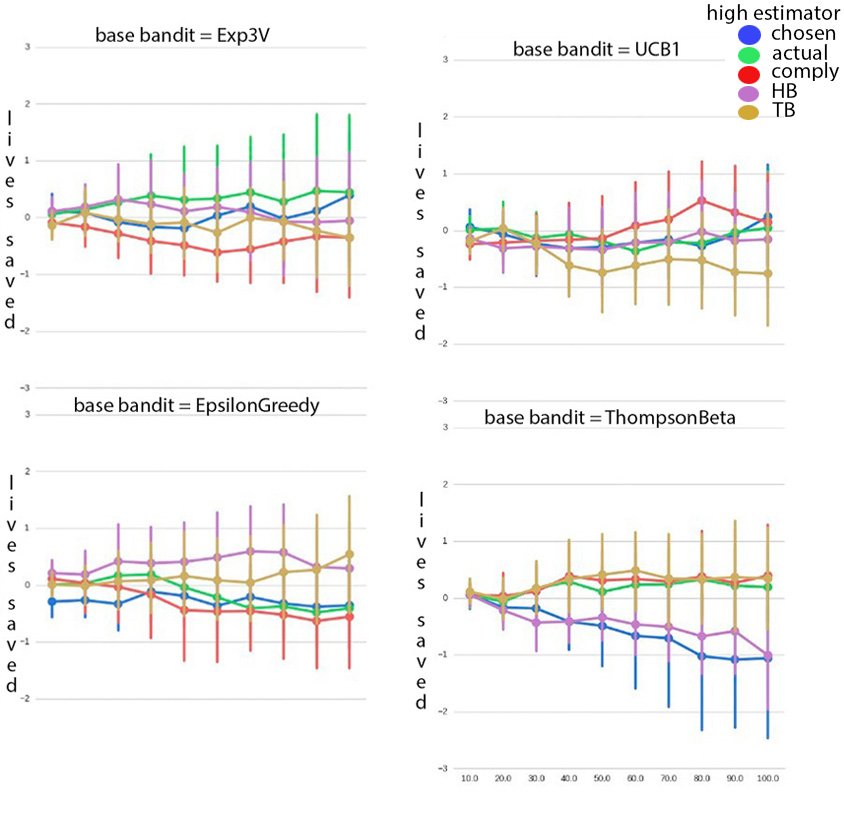
\includegraphics[width=1\columnwidth]{bandit/figs/fig1a.jpeg}
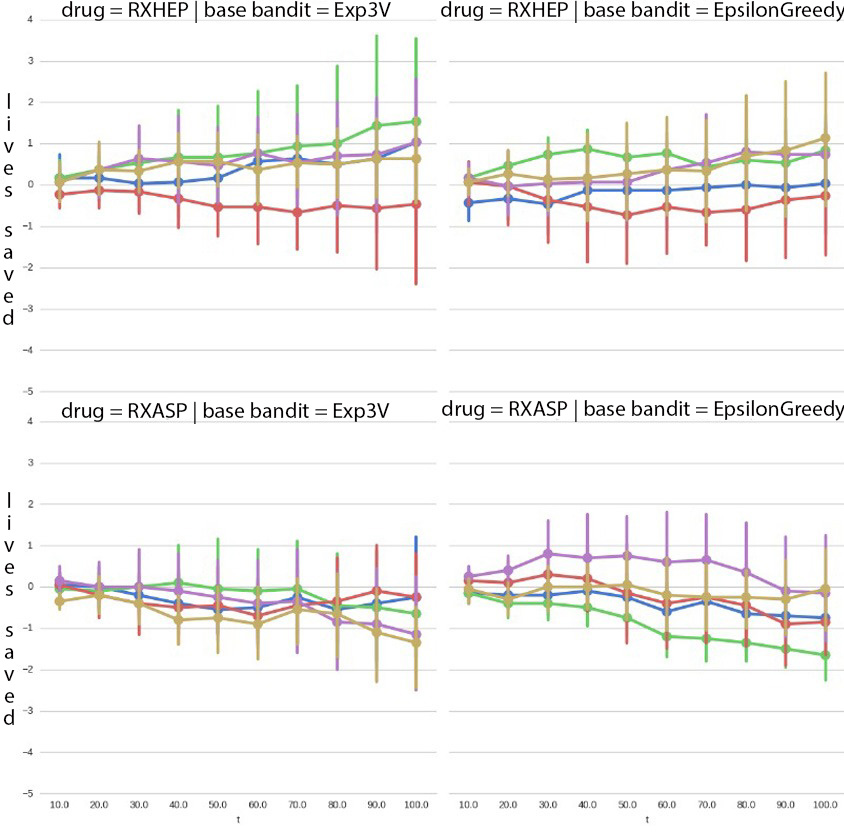
\includegraphics[width=1\columnwidth]{bandit/figs/fig1b.jpeg}
\caption{\textbf{14 Day survivals:} average lives saved over uniform random policy per 10,000 patients in 10,000 simulated trials of Aspirin and Heparin.}
\label{fig1}
\end{center}
\end{figure} 

We simulated 10,000 patients per run, which allowed us to not oversample the data in any single simulation; 2000 runs were performed, all algorithms were tested against the same draw of the run to minimize unnecessary sampling variation. 

The \texttt{EXP3} gamma parameter was set ahead of time to 0.085, a choice determined by the regret-bounds for $T=10000$ and $K=2$ or $3$. Epsilon-Greedy used a standard annealing schedule. No data dependent parameter tuning was used.
The simulation was carried out by creating a ``counter-factual patient'' by sampling (i.i.d.) one patient from each of the treatment and control groups in the clinical trial. If the algorithm selected the treatment, it then receives the reward and observes the action taken by the subject sampled form the treatment group, and vice versa for the control.


Empirically, \texttt{TB} achieved a surplus of 8.9 extra survivals (that is, human lives) with 95\% confidence interval $[8.1,9.7]$, relative to the randomized baseline.
\texttt{HB} with \texttt{Epsilon Greedy} as the base algorithm achieved a surplus of 9.2 (CI: $[8.3,10.0]$)
In contrast, the best performing strategy that was not compliance aware was Thompson sampling, which yielded 7.9 extra survivals (CI: $[7.2,8.7]$). 

The gains were largely concentrated in the Aspirin trial, which is consistent with the lack of benefits or severe ill effects found in the original study \cite{ist:97} for heparin, and with the small but beneficial effect found for aspirin. 
If the underlying treatment has no positive or negative effect, side-information after the fact alone cannot be helpful.
Note that \actual, and to a lesser extent \comply, performed better than either \chosen\, or the hybrid algorithms. However, these are problematic be used directly since no guarantees apply, their worst case performance unbounc. The performance of the hybrids benefits from the information encoded in \actual\, and \comply\, whilst keeping the guarantees of \chosen. 


A striking secondary finding is the strong interaction between the learning algorithm and the nature of the feedback used. In particular our naive implementation of \texttt{EXP3} performed extremely badly under both \actual\, and \comply, in both the aspirin and heparin simulations. As a result, it is remarkable is that \texttt{EXP3} performs well when used as a top-level algorithm in \texttt{HB} in both trials, and other algorithms on the same data with the same protocol are able to learn better than chosen, while \texttt{EXP3} does worse than random (note the \texttt{EXP3} guarantees are only for the \chosen\, protocol, so do not apply here).



\section{Synthetic Data}


To better understand the behavior of the algorithms in a more varied range of settings, we present results of simulations with synthetic data.
The first simulation illustrates example~2. For comparison, $T$ is kept at 10,000, and we simulated the binary outcome case. We assigned half the patients to rich and half to poor randomly. Rich patients always take the treatment and their outcome, which would otherwise be 1 with $p=1$, becomes 1 with  $p=0.75$. Poor patients only take the treatment when prescribed, their favorable outcome has probability $p=0.5$ without treatment; taking the treatment reduces the probability of a favourable outcome to $p=0.25$. Fig.~2 shows that the performance of \actual\, and \comply\, is much worse than \chosen\, and the hybrid algorithms.



\subsection{Selection of treatment on unobservables}

Consider a harmful treatment. Suppose there are two sub-populations with equal numbers of each. The first consists of rich, healthy patients who always take the treatment. The second consists of poor, less healthy patients who only take the treatment if prescribed. Finally, suppose the treatment reduces survival by 0.25. Assume that the right patients, if they didn't take the treatment would all do well (receive reward of 1), but they all take it, so face only a 0.75 chance of survival. Poor patients who face a baseline survival of 0.75, only take the treatment if instructed, which brings them down from 0.5. Results are for 100 samples.

%\input{tables/ex2}

%\input{figs/ex2}


\begin{figure}
	\centering	
	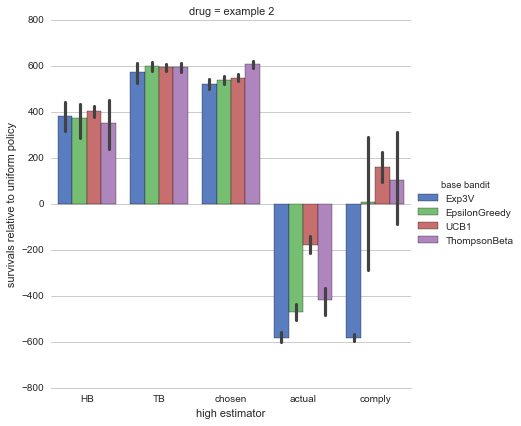
\includegraphics[width=1\columnwidth]{bandit/figs/ex2.jpeg}\hspace{1cm}
	\label{fig:ex2}
	\caption{Worse than random regret across estimators with naive uses of compliance awareness with simulated data from 100 simulations sampled from a model of a harmful treatment that is profound by selection into treatment.}
\end{figure}



\subsection{Small T}

The second simulation concerns small $T$. A motivation for very small $T$ adaptive clinical trials is provided by rare diseases. The overall size of the patient population is by construction severely restricted in this setting.
he priors for the mechanisms of action are also often poorly understood, so potential alternative treatments can have radically different probabilities of success. 
We simulate a $T=12$ adaptive trial with binary outcomes, with two treatments and expected rewards drawn uniformly from the unit interval, and compliance uniformly at random. We sample 1,000 such simulations.
A not uncommon size of clinical trials in rare diseases or neonatal populations
While our bounds are vacuous in this settings, it is interesting that there is on average an  improvement from taking the noncompliance information into account.


\begin{figure}[t]
	\centering	
	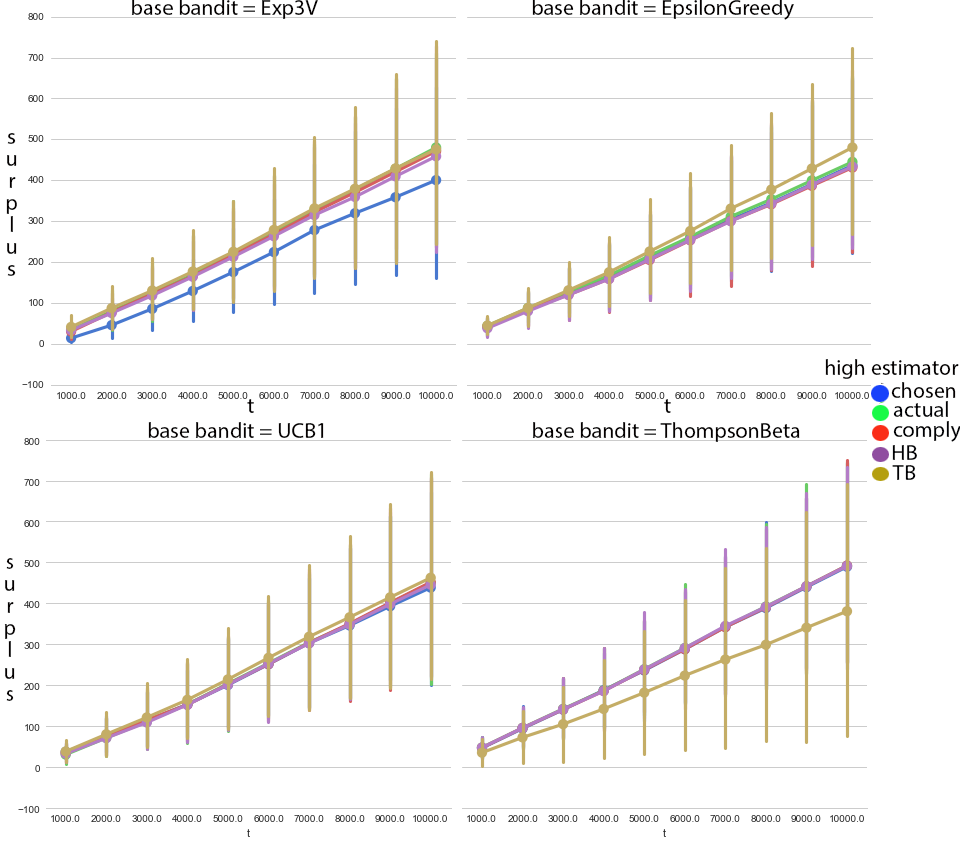
\includegraphics[width=0.9\textwidth]{bandit/figs/ex3.png}\hspace{1cm}
	\label{fig:ex3}
	\caption{Results from 1000 simulations with t=12 and synthetic data:with two treatments and expected rewards drawn uniformly from the unit interval, and compliance uniformly at random.}
\end{figure}





\subsection{Noncompliance for Best Arm}


A natural scenario for noncompliance and one that offers substantial potential is when the subject is better informed than the algorithm, and realizes they know a better alternative. 
This provides potentially huge practical advantages, specially in situations with very large numbers of a priori low expectation but high variance actions. 
They allow later subjects to benefit from the information that previous subjects bring to the mechanism, while current compliance unaware algorithms not only waste this information but hurt later subjects as it unnecessary raises the apparent variance of the rewards in the arms (since the chosen arm may indeed be very bad relative to the actual arm).




\begin{figure}[t]
	\centering	
	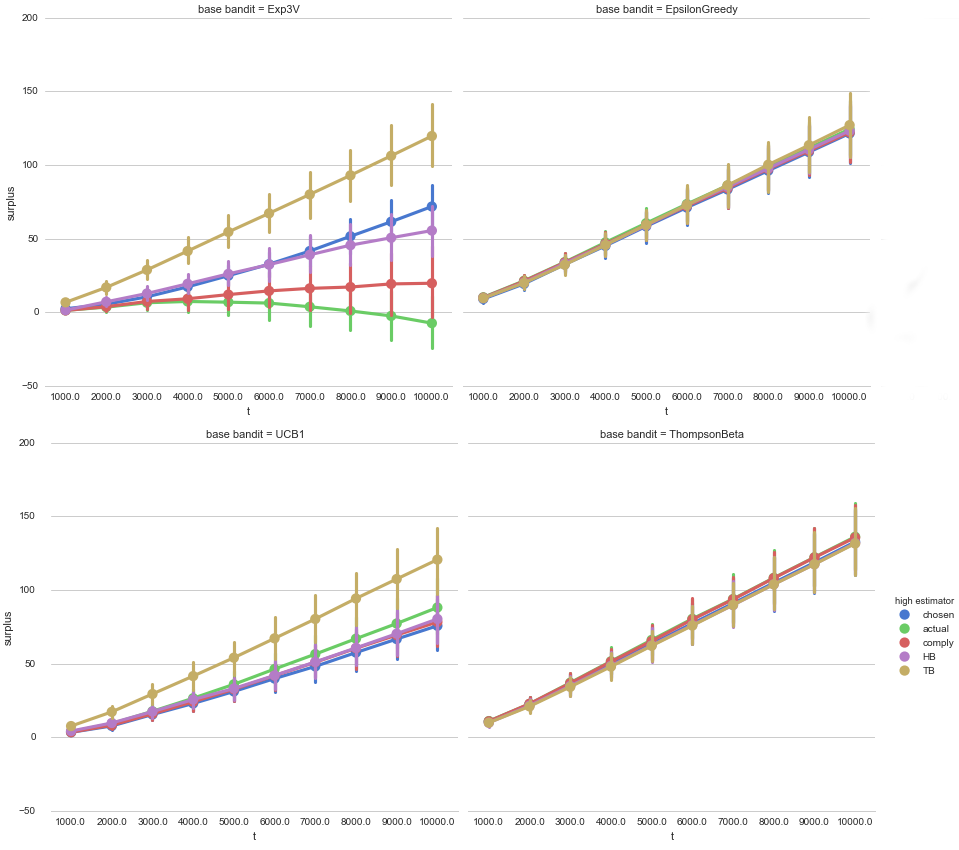
\includegraphics[width=0.9\textwidth]{bandit/figs/ex4.png}\hspace{1cm}
	\label{fig:ex4}
	\caption{Noncompliance for best arm: 100 simulations from synthetic data of T=10,000 with noncompliance proportional to how much better the best arm is than the algorithm selection.}
\end{figure}



%     def __init__(self,foo ):
%         n_arms=2
%         self.arm_value = 0.5+0.25*np.random.random(n_arms)
%         self.n_arms = n_arms
%     def draw_subject(self):
%         prefered_arm = stochastic_argmax(self.arm_value)
%         prefered_reward = random.binomial(1,self.arm_value[prefered_arm])
%         r = []
%         for i in range(self.n_arms):
%             if self.arm_value[i] / self.arm_value[prefered_arm] < random.random(): #informative noncompliance
%                 r.append((prefered_arm,prefered_reward))
%             else:  #compliers 
%                 r.append((i,  random.binomial(1,self.arm_value[i])))
%         return r

% example3= sim( nsim=100, T=10001, DGP=NoncomplianceForBestArm , drug="Better arm")
% display_results(example3.loc[example3['t'] == 10000].drop('t',1))



%\subsection{Independent Noncompliance and Rewards}

%We now simulate a neutral model, where compliance is unrelated to the rewards of the arm.
% #always or never takers. current simulation model is not rich enough for defiers, todo?
% class IndependentNoncomplianceAndRewards():
%     def __init__(self,foo):
%         n_arms=2
%         self.arm_value = 0.9+0.1*np.random.random(int(n_arms))
%         # todo add effect_magnitude=1
%         self.n_arms = n_arms
%     def draw_subject(self):
%         if random.random()<0.9: #compliers 
%             r=[(i, random.binomial(1,self.arm_value[i])) for i in range(self.n_arms)]
%         else:   #always takers
%             actual = categorical_draw(self.arm_value)
%             reward = random.binomial(1,self.arm_value[actual])
%             r= [(actual, reward) for i in range(self.n_arms)]
%         return r

    
% example4= sim( nsim=100, T=10001, DGP=IndependentNoncomplianceAndRewards , drug="example")
% display_results(example4.loc[example4['t'] == 10000].drop('t',1))







%think of the babies http://www.ncbi.nlm.nih.gov/pmc/articles/PMC2778326/



%We have two simulations, one in which noncompliance is independent of everything, and one where noncompliance is towards the higher expectation treatment.

%This is a boring figure, not rue what to say about it.
%%%%%%%%%%%%%%%%%%%%%%%%%%%%%%%%%%%%%%%%%%%%%%%%%%%%%%%%%%%%%%%%%%%%%%%%%%%%%%%%%%%%%%%%
%\subsection{Conclusions}

%Empirically, \texttt{TB} achieves a surplus of 8.9 extra survivals (that is, human lives) and \texttt{HB} achieves 9.2 surplus lives compared with 7.9 for the best classical algorithm. This suggests hybrid algorithms can make a significant difference to clinical outcomes.

% TODO, add note on composability and comparing to relatively well understood baselines. plug and play.

